\chapter{Admin}
Wesentlicher Bestandteil unseres Projektes war die Administrationsumgebung. Genauer musste eine Anwendung geschaffen werden, die dem jeweiligen Endanwender Navigationsdaten zur Verf�gung stellt. Also eine Umgebung, die einen Upload f�r Kartenmaterial bereitstellt. Des weiteren muss die Administrationsanwendung Features besitzen um Routen zu definieren und Meta-Informationen zu besonderen �rtlichkeiten festhalten zu k�nnen. Die Meta-Informationen k�nnen durch Points of Interest (PoI) Informationen erweitert werden.\\
Im folgenden Abschnitt wird zun�chst die allgemeine Struktur erl�utert und anschlie�end liegt das Hauptaugenwerk auf der Benutzeroberfl�che. Eine ausf�hrliche Bedienungsanleitung der Administrationsumgebung ist im Anhang beigef�gt.

\section{Allgemeine Struktur}
\subsection*{ASP.NET MVC 4}
Basis unserer Projektstruktur war das \textbf{ASP.NET MVC Framework}, welches ein Web Application Framework ist, und ein Model-View-Controller-Pattern implementiert.\\
Dies erm�glichte uns, eine Webanwendung zu entwickeln, bei der die Daten (\textit{Model}) gekapselt von der Ausgabe (\textit{View}) und dem \textit{Controller} vorliegen. Die \textit{View} repr�sentiert unsere Daten und der \textit{Controller} reagiert auf Zustands�nderungen und ist sozusagen das Bindeglied oder die Schnittstelle zwischen \textit{View} und \textit{Model}.

\subsection{Model}
\subsubsection*{AccountModels}
Kapselt die benutzerspezifischen Daten in einem Model zur Authentifizierung von Benutzerprofilen. Dieses Model findet Verwendung beim Registrieren sowie beim LogIn- / LogOut-Verfahren.
\subsubsection*{AdminModels}
Model indem der MapName gekapselt vorliegt.
\subsubsection*{FloorViewModel}
Dieses Model enth�lt Daten zu einem Floor. FloorId, MapId und FloorImageFile sind diese Daten.
\subsubsection*{MapViewModel}
MapId und Name werden f�r die MapView in diesem Model gekapselt.

\subsection{View}
Die Views in unserem Projekt wurden in Views die den Account-, den Admin- und den Home-Bereich betreffen unterteilt.
\subsubsection*{Account}
Enth�lt html-Seiten zum registrieren, anmelden und verwalten den eigenen Benutzerprofils.
\subsubsection*{Admin}
Unter dieser Rubrik fallen die Webseiten, mit dem der Administrator Maps, Floors und Knoteninformationen zu einer Map hinzuf�gen kann. Sozusagen die Arbeitsoberfl�che des Administrators.
\subsubsection*{Home}
Einstiegspunkt oder oberstes Element (Index) unserer Webseite.

\subsection{Controller}
\subsubsection*{HomeController}
Speziell f�r unser Projekt bedeutet es, dass wir drei Controller angelegt haben. Der Einstiegspunkt unserer Web-Anwendung ist der sogenannte \textit{HomeController}. Dies ist der Controller, der zum Zuge kommt, sofern die anderen beiden Controller eine Interaktion oder Controller-Aufrufe mit gewissen Parametern nicht unterst�tzen.
\subsubsection*{AccountController}
Der \textit{AccountController} verarbeitet die Ereignisse, die vom Registrierungs-, LogIn- und LogOut-Verhalten eines Benutzers ausgel�st werden. Im Fokus stehen hierbei die \textbf{HTTP GET-} und \textbf{HTTP POST-Methoden}, die von der Klasse \textit{AccountController} implementiert werden.
\subsubsection*{AdminController}
Der \textit{AdminController} reagiert auf Zustands�nderungen, die beim Anlegen, Bearbeiten und L�schen von Datenmaterial in Form von Karten oder Informationen (Meta-Informationen), ausgel�st werden.\\
Relevante Funktionen sind die Methoden zum erstellen und l�schen von Maps und Floors.
Des weiteren werden �ber diesen Controller die Routeninformationen als Graph verarbeitet und in einer Datenbank gespeichert. Detailinformationen zu einem Knoten aus einem Graphen verarbeitet dieser Controller und speichert sie ab. Diese Detailinformationen erm�glichen besondere Orte als \textit{Points of Interest} zu kennzeichnen.

\section{Benutzeroberfl�che}
Die Administrator Benutzeroberfl�che ist �ber folgenden Link \\
\href{URL}{http://193.175.199.115/StudMapAdmin/} erreichbar.
\begin{figure}[H]
\centering
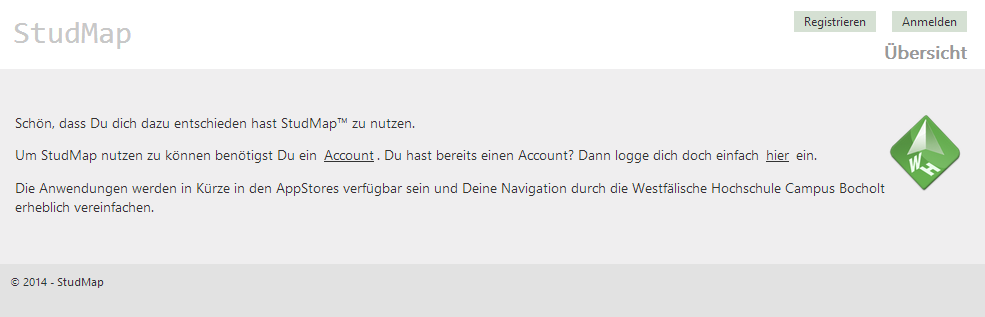
\includegraphics[width=\linewidth]{../Bilder/Admin/AdminHome}
\label{fig:AdminHome}
\end{figure}
Der Anwender enth�lt die M�glichkeit sich anzumelden oder sich zu registrieren.
\subsubsection*{Registrieren}
\href{URL}{http://193.175.199.115/StudMapAdmin/Account/Register}
\begin{figure}[H]
\centering
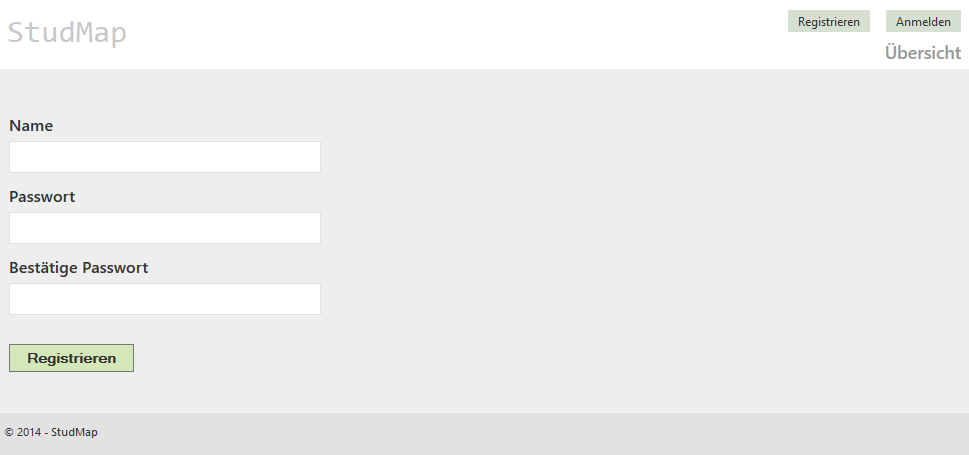
\includegraphics[width=\linewidth]{../Bilder/Admin/AdminRegistrierung}
\label{fig:AdminRegistrierung}
\end{figure}
\subsubsection*{Anmelden}
\href{URL}{http://193.175.199.115/StudMapAdmin/Account/Login}
\begin{figure}[H]
\centering
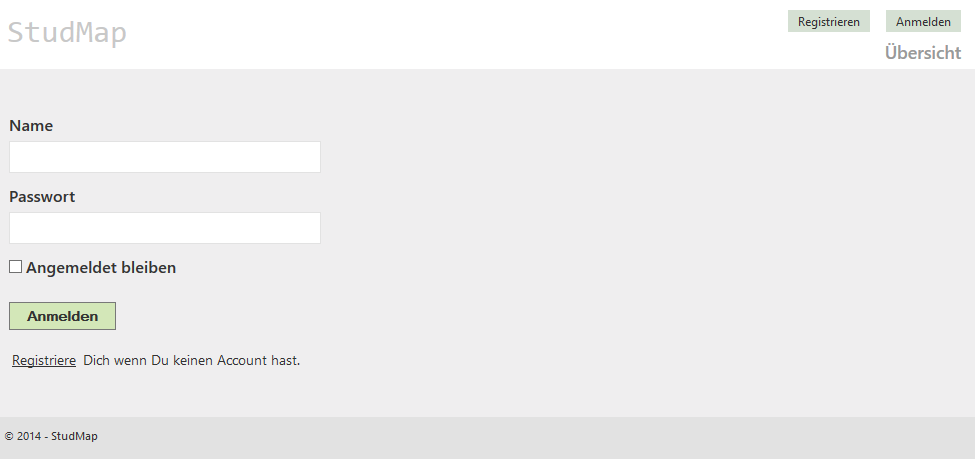
\includegraphics[width=\linewidth]{../Bilder/Admin/AdminAnmelden}
\label{fig:AdminAnmelden}
\end{figure}

\subsubsection*{Admin}
Den Einstiegspunkt zum verwalten von Maps finden Sie unter folgenden Link \\
\href{URL}{http://193.175.199.115/StudMapAdmin/Admin}. Er enth�lt eine Auflistung aktuell vorhandener Maps. Es  k�nnen neue Maps erstellt, bzw. vorhandene entfernt werden.
\begin{figure}[H]
\centering
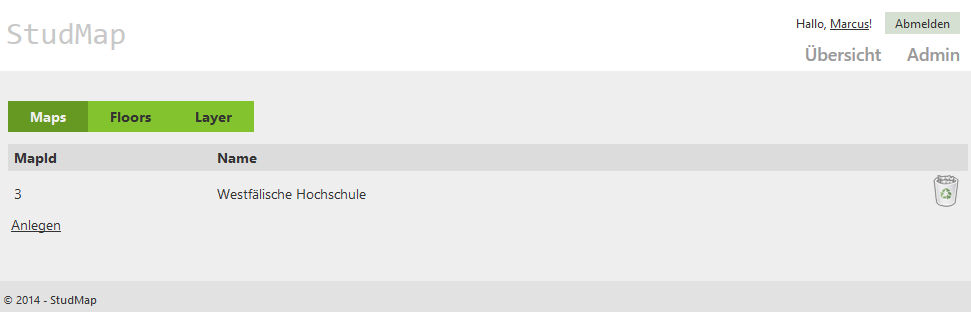
\includegraphics[width=\linewidth]{../Bilder/Admin/AdminMaps}
\label{fig:AdminMaps}
\end{figure}
Die Verwaltung der einzelnen Floors zu einer Map werden in der nachfolgenden Grafik gezeigt. Durch einen Klick auf \textit{Anlegen} kann eine neue Floor, mit der zugeh�rigen Kartengrundlage hinzugef�gt werden.
\begin{figure}[H]
\centering
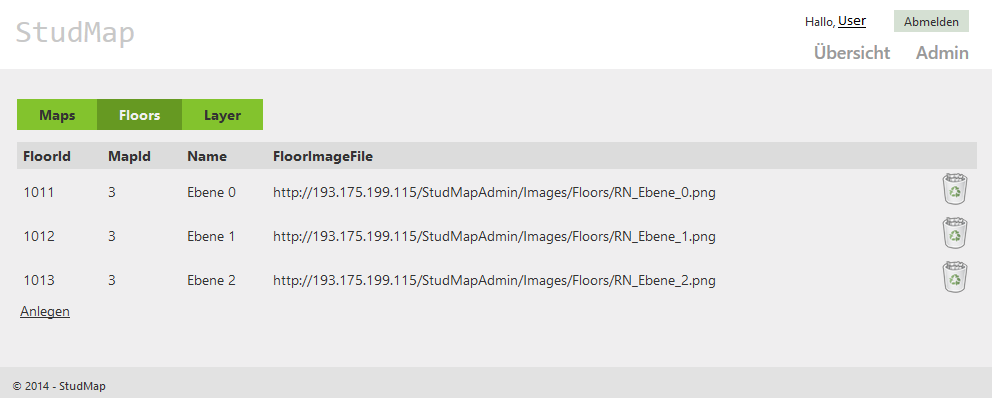
\includegraphics[width=\linewidth]{../Bilder/Admin/AdminFloors}
\label{fig:AdminFloors}
\end{figure}
Der Layer zeigt die Karte und einen gegebenenfalls erstellten Graphen mit Knoten und Kanten zu genau einem Floor an.
Durch Verwendung spezieller Features kann der Administrator hier einen Graphen erstellen und Knoteninformationen hinterlegen. Des weiteren besteht die M�glichkeit Knoten mit Knoten anderer Floors zu verkn�pfen. Basis f�r eine ergonomische Navigation der Karte ist die JavaScript-Bibliothek D3.
\begin{figure}[H]
\centering
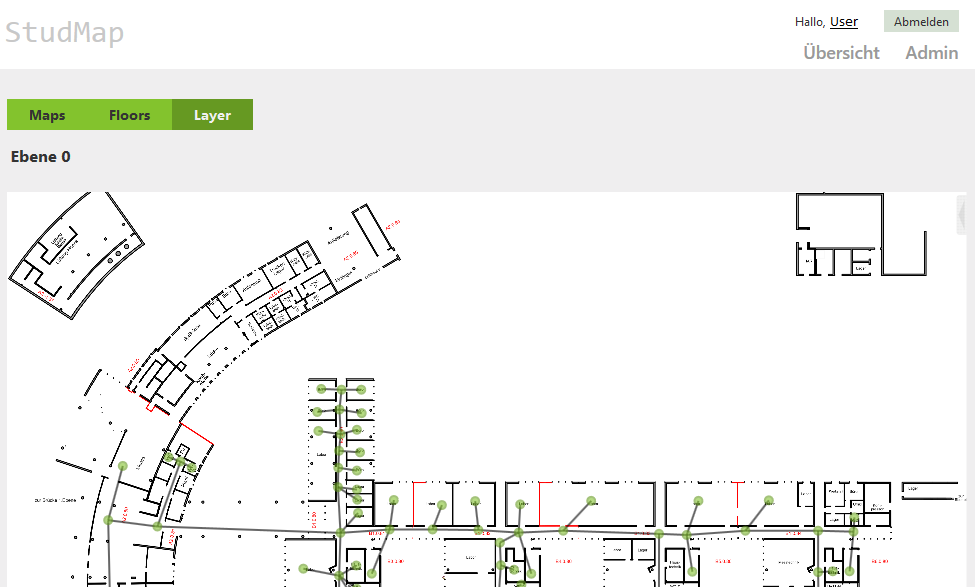
\includegraphics[width=\linewidth]{../Bilder/Admin/AdminLayer}
\label{fig:AdminLayer}
\end{figure}
\begin{figure}[H]
\centering
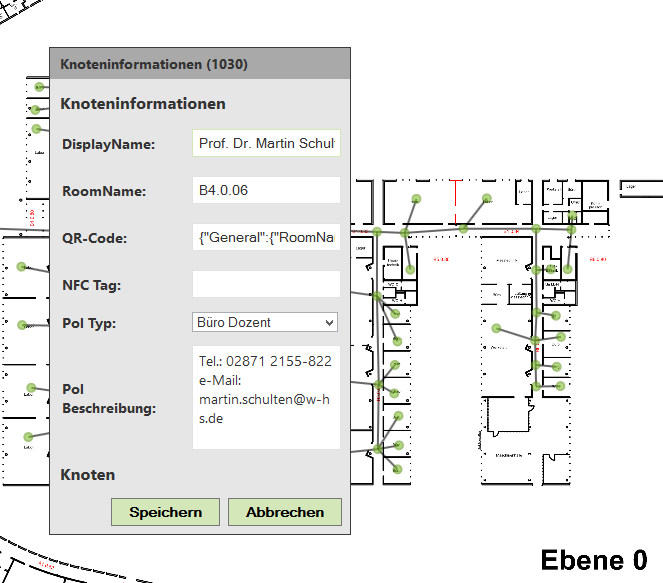
\includegraphics[width=\linewidth]{../Bilder/Admin/AdminNodeInfo}
\label{fig:AdminNodeInfo}
\end{figure}
�ber den Button \textit{Abmelden} gelangen Sie zum Index unserer Webseite zur�ck.

\section{Admin Spezifisches}
\subsection*{Neuen Benutzer mit Administrator Rechten versehen}
\label{Administrator Rechte versehen}
Nachdem ein neuer Benutzer die Registratur erfolgreich abgeschlossen hat, ist dieser im Benutzerprofil noch nicht als Administrator gekennzeichnet. Derzeit ist es so, dass ein Datenbankadministrator in der Tabelle \textit{webpages\_UsersInRoles} den Eintrag von 1 f�r Users auf 2 f�r Admins ab�ndern muss. Nur Admins haben die Rechte Maps und Floors zu erstellen, sowie das Kartenmateral mit Metainformationen zu bereichern.
\subsection*{ELMAH}
Als Logging Werkzeug haben wir das auf der .NET Plattform sehr verbreitete und OpenSource Tool \textit{ELMAH} eingesetzt. \textit{ELMAH}\footnote{ELMAH steht f�r "Error Logging Modules and Handlers"} loggt auftretende Fehler und Exceptions. Nach kurzem Installationsaufwand und Konfiguration einer Datenbank, in der die Fehler gespeichert werden, kann das Tool bereits genutzt werden. Genaue Installationsanleitungen findet Sie zu gen�ge im 
Internet\footnote{\href{URL}{http://blog.thomasbandt.de/39/2380/de/blog/elmah-mit-aspnet-mvc-nutzen-und-fehler-loggen.html}}. 

\section{Maintenance Tool}
W�hrend der Entwicklung des StudMap-Projektes ist es uns aufgefallen, dass wir 
zur Wartung und Ausf�hrung bestimmter Aufgaben ein einfaches Tool hilfreich 
w�re. Daher haben wir eine WPF-Anwendung entwickelt, welche die folgenden 
Aufgaben erledigt.

\section{QR-Codes generieren}
Eine M�glichkeit der Positionierung innerhalb des StudMap-Projektes ist das 
Einlesen von QR-Codes. In diesen QR-Codes stehen die im Kapitel 
\nameref{QR-Tags} beschriebenen Daten.\\
In der Anwendung werden alle \nameref{object:NodeInformation} ausgelesen und 
in einer Tabelle angezeigt. Anschlie�end kann in dieser Tabelle noch nach 
einem \nameref{object:Floor}, oder dem Namen des Raums gefiltert werden.\\
Abschlie�end kann f�r alle ausgew�hlten Knoten ein QR-Code als PNG generiert 
werden. Zur Generierung der QR-Codes nutzen wir die Bibliothek 
\href{http://qrcodenet.codeplex.com/}{QrCode.Net}.

% TODOS:
% - Funktionsweise (Knoten �ber zwei Ebenen miteinander verbinden)
% - UI Aspekte (x)
% - MVC Web Zeug... (x)
% - Verweis auf Anhang f�r Bedienungsanleitung / Installationsanleitung